\chapter{O$_2$ Module}

The O$_2$ module is a simple oxygen evolution module,
intermediate between the Streeter and Phelps
\cite{streeter_ohio_1925} model,
which is restricted to modeling reaeration and the global oxidizable load,
and a more complete module, such as EUTRO, simulating several oxidation processes
and explicitly computes the phytoplankton evolution and its influence on oxygen.
The O$_2$ model advantage is its simplicity
(eight parameters to calibrate, excluding parameterization of weirs).
Some important parameters are assumed constant, such as benthic demand or plant respiration.
The use of the model is consequently limited to phenomena of a few days duration,
such as reservoir emptying. Three tracers are involved:

\begin{itemize}
\item dissolved oxygen O$_2$ (mgO$_2$/l),
\item the organic load L (mgO$_2$/l),
\item the ammonia load NH4 (mgH$_4$/l).
\end{itemize}

These variables are advected and dispersed in the water mass accordingly
to the advection-dispersion equation, with external and internal sources.
Six factors influencing the concentration of dissolved oxygen are considered:

\begin{itemize}
\item four factors consuming oxygen: organic load, ammonia load,
  benthic demand and plant respiration,
\item two processes creating oxygen: photosynthesis and reaeration.
\end{itemize}

The terms dealing with internal sources of each considered tracer are explained
in the following sections.

\section{Dissolved oxygen}

\subsection{Benthic demand}

The benthic demand $BEN$ is provided by the user in gO$_2$/m$^2$/d.
It is adjusted according to the temperature $T$ as:

\begin{equation}
  BEN_T = BEN_{20^\circ \rm{C}} (1.065)^{T-20}.
\end{equation}

The following Table gives some typical values of benthic demand
at $T$ = 20$^\circ$C (i.e. $BEN_{20^\circ \rm{C}}$).\\

\begin{table}[H]
 			\centering
\begin{tabular}{p{3.0in}p{3.0in}}
\hline
%row no:1
\multicolumn{1}{|p{3.0in}}{Bottom type} & 
\multicolumn{1}{|p{3.0in}|}{Typical value of $BEN$ (gO$_2$/m$^2$/d) at 20$^{\circ}$C} \\
\hline
%\hhline{--}
%row no:2
\multicolumn{1}{|p{3.0in}}{Filamentous bacteria (10~g/m$^2$)} & 
\multicolumn{1}{|p{3.0in}|}{7} \\
\hline
%\hhline{--}
%row no:3
\multicolumn{1}{|p{3.0in}}{Mud from waste water, near to release} & 
\multicolumn{1}{|p{3.0in}|}{4} \\
\hline
%\hhline{--}
%row no:4
\multicolumn{1}{|p{3.0in}}{Mud from waste water, far from release } & 
\multicolumn{1}{|p{3.0in}|}{1.5} \\
\hline
%\hhline{--}
%row no:5
\multicolumn{1}{|p{3.0in}}{Estuarine silt} & 
\multicolumn{1}{|p{3.0in}|}{1.5} \\
\hline
%\hhline{--}
%row no:6
\multicolumn{1}{|p{3.0in}}{Sand} & 
\multicolumn{1}{|p{3.0in}|}{0.5} \\
\hline
%\hhline{--}
%row no:7
\multicolumn{1}{|p{3.0in}}{Mineral soil} & 
\multicolumn{1}{|p{3.0in}|}{0.007} \\
\hline
%\hhline{--}

\end{tabular}
\end{table}

\subsection{Plant respiration}

The plant respiration $R$ (in mgO$_2$/d/l) is provided by the user.

\subsection{Photosynthesis}

The photosynthesis $P$ (in mgO$_2$/d/l) depends on algae, water depth and light,
with order of magnitude between 0.3 mgO$_2$/l/d and 9 mgO$_2$/l/d
depending on the flow discharge \cite{streeter_ohio_1925}.
In the O$_2$ model, $P$ is provided by the user.

\subsection{Reaeration}

\subsubsection{Natural reaeration}

Reaeration is an oxygen supply through the free surface.
At macroscopic scale, it can be modeled as linearly proportional to ($C_s$ - [O$_2$]),
where $C_s$ is the oxygen concentration at saturation in the water (in mgO$_2$/l)
(Reminder: $C_s$ = 9 mg/l at 20$^{\circ}$C). Therefore:

\begin{equation}
  Reaeration = k_2 \left( C_s - [\rm{O}_2] \right).
\end{equation}

The coefficient $k_2$ (d$^{-1}$) is a parameter with
orders of magnitude indicated in the Table below
(from \cite{tchobanoglous_wq_1985}).\\

\begin{table}[H]
 			\centering
\begin{tabular}{p{3.0in}p{3.0in}}
\hline
%row no:1
\multicolumn{1}{|p{3.0in}}{Type of watercourse} & 
\multicolumn{1}{|p{3.0in}|}{Interval of $k_2$ (d$^{-1}$) at 20$^{\circ}$C} \\
\hline
%\hhline{--}
%row no:2
\multicolumn{1}{|p{3.0in}}{Small ponds and backwaters} & 
\multicolumn{1}{|p{3.0in}|}{0.10-0.23} \\
\hline
%\hhline{--}
%row no:3
\multicolumn{1}{|p{3.0in}}{Sluggish streams and large lakes} & 
\multicolumn{1}{|p{3.0in}|}{0.23-0.35} \\
\hline
%\hhline{--}
%row no:4
\multicolumn{1}{|p{3.0in}}{Large streams of low flow velocity} & 
\multicolumn{1}{|p{3.0in}|}{0.35-0.46} \\
\hline
%\hhline{--}
%row no:5
\multicolumn{1}{|p{3.0in}}{Large streams of normal flow velocity} & 
\multicolumn{1}{|p{3.0in}|}{0.46-0.69} \\
\hline
%\hhline{--}
%row no:6
\multicolumn{1}{|p{3.0in}}{Swift streams} & 
\multicolumn{1}{|p{3.0in}|}{0.69-1.15} \\
\hline
%\hhline{--}
%row no:7
\multicolumn{1}{|p{3.0in}}{Rapids and waterfalls} & 
\multicolumn{1}{|p{3.0in}|}{> 1.15} \\
\hline
%\hhline{--}

\end{tabular}
\end{table}

There are plenty of formulae calculating $k_2$,
which indicates the low level of our understanding of this process.
We can distinguish conceptual formulae,
valid only within limited conditions,
and semi-empirical and empirical formulae
that are valid where conditions are not too far from those of calibration.
Actually, there is little difference between the formulae when the water depth
is between 0.3~m and 3~m.
The O$_2$ model allows using four formulae cited in \cite{mccutcheon_wq_1989}:

\begin{equation}
  k_2 = 5.23 U h^{-1.67} \quad \rm{(Tennessee~Valley~Authority)},
\end{equation}

\begin{equation}
  k_2 = 5.33 U^{0.67} h^{-1.85} \quad \rm{(Owens~et~al.)},
\end{equation}

\begin{equation}
  k_2 = 0.746 U^{2.695} h^{-3.085} J^{-0.823} \quad \rm{(Churchill~et~al.)},
\end{equation}

\begin{equation}
  k_2 = 3.9 U^{0.5} h^{-1.5} \quad \rm{(O’Connor~and~Dobbins)},
\end{equation}

with $U$ is the magnitude of velocity (in m/s)
and $J$ is the energy slope (in m).

The O’Connor and Dobbins formula provides the best results for shallow rivers.
For deep and rapid rivers, Churchill et al.'s formula is preferable.
Figure \ref{validity_domain_reaeration} shows the areas of application for selected formulae
\cite{mccutcheon_wq_1989}:

\begin{figure}[H]
  \centering
  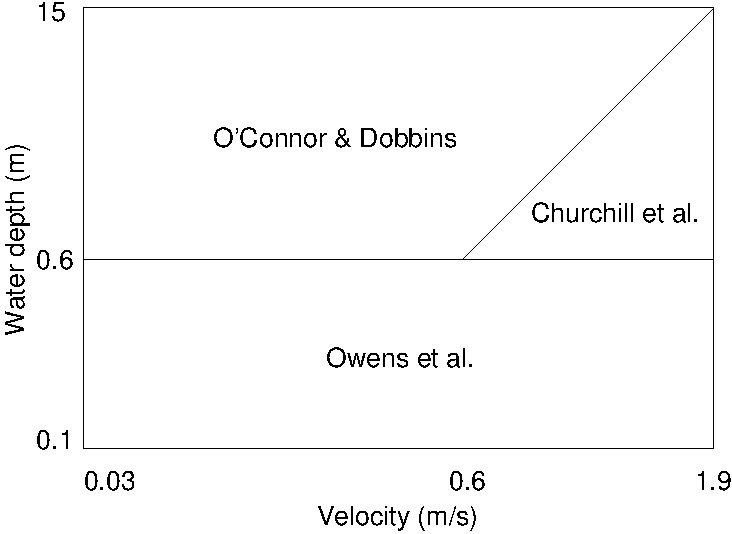
\includegraphics[scale=0.3]{graphics/validity_domain_reaeration_O2.png}
  \caption{Application areas of Owens et al., Churchill et al. and O'Connor
    and Dobbins formulae \cite{mccutcheon_wq_1989}.}
  \label{validity_domain_reaeration}
\end{figure}

One option allows the user fixing a value for $k_2$.
Another option allows choosing one of the four formulae described above.
The value of $k_2$, valid at 20$^{\circ}$C, is adjusted according to the temperature as:

\begin{equation}
  k_2 = (k_2)_{20^{\circ}\rm{C}} (1.0241)^{T-20}.
\end{equation}

The oxygen concentration at saturation in the water $C_s$ can be determined
according to the water temperature (at 20$^{\circ}$C, $C_s$ = 9 mgO$_2$/l).
This is a parameter that must be known and can be calculated
if connected to a temperature module such as THERMIC.
Elmore and Hayes (cited in \cite{mccutcheon_wq_1989}) proposed the following formula
(with $T$ in $^{\circ}$C) for calculating $C_s$:

\begin{equation}
  C_s = 14.652 - 0.41022 T + 0.007991 T^2 - 7.7774.10^{-5}T^3.
\end{equation}

More recent models include a correction for atmospheric pressure and, in estuaries, for salinity.
However, we consider that we are far from estuarial conditions and the variations in pressure
entail insignificant variations in dissolved oxygen compared to those that we need.
Montgomery et al.'s equation (cited in \cite{mccutcheon_wq_1989})
only deviates from standard formulae by $ \pm $  0.02 mgO$_2$/l
between 0 and 50$^{\circ}$C when there is negligible salinity.

\begin{equation}
  C_s = \frac{468}{31.6+T}.
\end{equation}

The model allows choosing either a fixed $C_s$ value given
by the user or by one of the two formulae described above.\\

\subsubsection{Reaeration due to weirs (not used at the moment in WAQTEL)}

A weir can provide between 1 and 3 mg/l of dissolved oxygen \cite{mccutcheon_wq_1989}.
The ratio $r$ is defined by the relationship $$r = \frac{C_s-C_u}{C_s-C_d},$$

with $C_u$ = oxygen concentration upstream of weir,
$C_d$ = oxygen concentration downstream of weir.
The knowledge of $C_u$ and $r$  enables calculating $C_d$.
$C_d$ is directly applied.
This term therefore is not treated as a source.
The rate $r$ can be determined empirically
\cite{mccutcheon_wq_1989}: e.g.,

\begin{equation}
  r = 1 + 0.5 a b \Delta h \quad \rm{(Gameson)},
\end{equation}

\begin{equation}
  r = 1+ 0.36 a b (1+0.046 T) \Delta h \quad \rm{(Gameson~et~al.)},
\end{equation}

\begin{equation}
  r = 1 + 0.69 \Delta h (1 - 0.11 \Delta h) (1 +0.046 T) \quad \rm{(Water~Research~Laboratory)},
\end{equation}

\begin{equation}
  r = 1 + 0.38 a b  \Delta h (1 - 0.11 \Delta h) (1 +0.046 T),
  \quad \rm{(Water~Research~Laboratory)}
\end{equation}

with $a$ = measure of water quality (= 0.65 for highly polluted streams,
= 1.8 for clear streams),
$b$ = characteristic parameter of the weir,
$\Delta h$ = water level difference between upstream and downstream of the weir.
The following Table gives $b$ values for different weirs \cite{mccutcheon_wq_1989}:\\

\begin{table}[H]
 			\centering
\begin{tabular}{p{3.0in}p{3.0in}}
\hline
%row no:1
\multicolumn{1}{|p{3.0in}}{Type of weir} & 
\multicolumn{1}{|p{3.0in}|}{$b$} \\
\hline
%\hhline{--}
%row no:2
\multicolumn{1}{|p{3.0in}}{flat broad-crested regular step} & 
\multicolumn{1}{|p{3.0in}|}{0.7} \\
\hline
%\hhline{--}
%row no:3
\multicolumn{1}{|p{3.0in}}{flat broad-crested irregular step} & 
\multicolumn{1}{|p{3.0in}|}{0.8} \\
\hline
%\hhline{--}
%row no:4
\multicolumn{1}{|p{3.0in}}{flat broad-crested vertical face} & 
\multicolumn{1}{|p{3.0in}|}{0.8} \\
\hline
%\hhline{--}
%row no:5
\multicolumn{1}{|p{3.0in}}{flat broad-crested straight slope face} & 
\multicolumn{1}{|p{3.0in}|}{0.9} \\
\hline
%\hhline{--}
%row no:6
\multicolumn{1}{|p{3.0in}}{flat broad-crested curved face} & 
\multicolumn{1}{|p{3.0in}|}{0.75} \\
\hline
%\hhline{--}
%row no:7
\multicolumn{1}{|p{3.0in}}{round broad-crested curved face} & 
\multicolumn{1}{|p{3.0in}|}{0.6} \\
\hline
%\hhline{--}
%row no:8
\multicolumn{1}{|p{3.0in}}{sharp-crested straight slope face} & 
\multicolumn{1}{|p{3.0in}|}{1.05} \\
\hline
%\hhline{--}
%row no:9
\multicolumn{1}{|p{3.0in}}{sharp-crested vertical face} & 
\multicolumn{1}{|p{3.0in}|}{0.8} \\
\hline
%\hhline{--}
%row no:10
\multicolumn{1}{|p{3.0in}}{sluice gates with submerged discharge} & 
\multicolumn{1}{|p{3.0in}|}{0.05} \\
\hline
%\hhline{--}

\end{tabular}
\end{table}

In the model, $r$ can be either a fixed value given by the user or
calculated by one of the 4 formulae previously described.\\

\section{Organic load}

The organic load $L$ (in mgO$_2$/l) is a variable evolving over time
from an initial condition according to a 1$^{\rm{st}}$ order law:

\begin{equation}
  F([L]) = -k_1 [L],
\end{equation}

where $k_1$ is the kinetic degradation constant of the organic load (d$^{-1}$).
It is a parameter of the model.
In the O$_2$ model, the organic load $L$ is considered to be an independent variable.

\section{Ammonia load}

Also consuming oxygen, the variable ammonia load NH$_4$ (in mgH$_4$/l) follows
a 1$^{\rm{st}}$ order decay law

\begin{equation}
  F([NH_4]) = -k_4 [NH_4],
\end{equation}

where $k_4$ the kinetic constant of nitrification (d$^{-1}$),
a parameter of the model.
In the O$_2$ model, the ammonia load is considered to be an independent variable.\\

\section{Solved equation}

The concentration of dissolved oxygen [O$_2$] (in mgO$_2$/l) changes
according to the effect of sources:

\begin{equation}
  F([O_2]) = k_2 (C_s - [O_2]) -k_1 [L] - k_4 [NH_4] + P - R - \frac{BEN_T}{h}.
\end{equation}

Using the terminology and notations of section \ref{waq_models}
and setting $C_1$ = [O$_2$], $C_2$ = [L] and $C_3$ = [NH$_4$],
the matrices [$ \lambda $] and [$ \mu $]
%containing the coefficients $\lambda_i^j$ and $ \mu_i^j$
are written as:\\

$$  [\lambda] = \frac{1}{86400}
  \begin{pmatrix}
    -k_2 & -k_1  & -k_4 \\
     0   & -k_1  & 0    \\
     0   &  0    & -k_4
  \end{pmatrix}
$$
  
$$
  [\mu] = 
  \begin{pmatrix}
     0  & 0 & 0 \\
     0  & 0 & 0 \\
     0  & 0 & 0
  \end{pmatrix}
$$  

(Note: Division by 86,400 scales down the time to one second).\\

The only non-zeros terms $ \lambda_1^0$ and $ \mu_1^0$ are:

\begin{equation}
  \lambda_1^0 = \frac{k_2 C_s + P - R}{86400},
\end{equation}

\begin{equation}
  \mu_1^0 = -\frac{BEN_T}{86400}.
\end{equation}
